\documentclass[A4,12pt, utf8]{article}
\usepackage{tikz}
\usepackage[
    backend=biber,
    style=authoryear-icomp,
    sortlocale=de_DE,
    natbib=true,
    url=false, 
    doi=true,
    eprint=false
]{biblatex}
\usepackage{listings}
\usepackage{xcolor}
\usepackage{hyperref}
\usepackage{pgf}
\usepackage{tikz}
\usetikzlibrary{arrows,automata}
\usepackage{todonotes}
\usepackage{dirtree}
\usepackage{pdflscape}
\usepackage{csquotes}
\MakeOuterQuote{"}


\newcommand{\tinytodo}[2][]
   {\todo[caption={#2}, size=\small, #1]{\renewcommand{\baselinestretch}{0.5}\selectfont#2\par}}

\colorlet{punct}{red!60!black}
\definecolor{background}{HTML}{EEEEEE}
\definecolor{delim}{RGB}{20,105,176}
\colorlet{numb}{magenta!60!black}

\lstdefinelanguage{json}{
    basicstyle=\normalfont\ttfamily,
    % numbers=left,
    % numberstyle=\scriptsize,
    % stepnumber=1,
    % numbersep=8pt,
    showstringspaces=false,
    breaklines=true,
    frame=lines,
    backgroundcolor=\color{background},
    literate=
     *{0}{{{\color{numb}0}}}{1}
      {1}{{{\color{numb}1}}}{1}
      {2}{{{\color{numb}2}}}{1}
      {3}{{{\color{numb}3}}}{1}
      {4}{{{\color{numb}4}}}{1}
      {5}{{{\color{numb}5}}}{1}
      {6}{{{\color{numb}6}}}{1}
      {7}{{{\color{numb}7}}}{1}
      {8}{{{\color{numb}8}}}{1}
      {9}{{{\color{numb}9}}}{1}
      {:}{{{\color{punct}{:}}}}{1}
      {,}{{{\color{punct}{,}}}}{1}
      {\{}{{{\color{delim}{\{}}}}{1}
      {\}}{{{\color{delim}{\}}}}}{1}
      {[}{{{\color{delim}{[}}}}{1}
      {]}{{{\color{delim}{]}}}}{1},
}
% \addbibresource{linked.bib}

\newcounter{treeline}

\newcommand{\treeroot}[1]{% Title
\node[above] at (0,0) {#1};%
\setcounter{treeline}{0}
}

\newcommand{\treeentry}[2]{% Title, Level
\draw[->] (#2-1,-\value{treeline}/2) -- (#2-1,-\value{treeline}/2-0.5) -- (#2+0.5,-\value{treeline}/2-0.5) node[right] {#1};
\stepcounter{treeline}
}

\newcommand{\altentry}[2]{% Title, Level
\draw[->] (#2-1,-\value{treeline}/2) -- (#2-1,-\value{treeline}/2-0.5) -- (#2+0.5,-\value{treeline}/2-0.5) node[right] {#1};
\foreach \x in {1,...,#2}
{   \draw (\x-1,-\value{treeline}/2) -- (\x-1,-\value{treeline}/2-0.5);
}
\stepcounter{treeline}
}


\title{emuLVC - Stucture of the angularjs app}
\author{Raphael Winkelmann}
\date{\today}
\begin{document}
  % \maketitle

\section{Schematic DB file structure on disc}

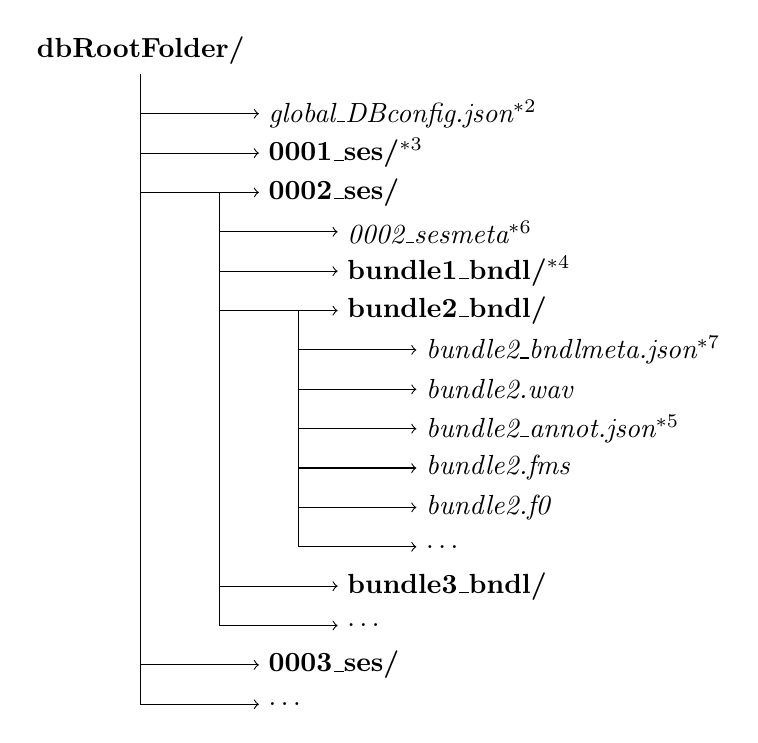
\begin{tikzpicture}
\treeroot{\textbf{dbRootFolder/}}
\altentry{\textit{global\_DBconfig.json$^{*2}$}}{1}
\altentry{\textbf{0001\_ses/$^{*3}$}}{1}
\altentry{\textbf{0002\_ses/}}{1}
\altentry{\textit{0002\_sesmeta$^{*6}$}}{2}
\altentry{\textbf{bundle1\_bndl/$^{*4}$}}{2}
\altentry{\textbf{bundle2\_bndl/}}{2}
\altentry{\textit{bundle2\_bndlmeta.json$^{*7}$}}{3}
\altentry{\textit{bundle2.wav}}{3}
\altentry{\textit{bundle2\_annot.json$^{*5}$}}{3}
\altentry{\textit{bundle2.fms}}{3}
\altentry{\textit{bundle2.f0}}{3}
\altentry{\dots}{3}
\altentry{\textbf{bundle3\_bndl/}}{2}
\altentry{\dots}{2}
\altentry{\textbf{0003\_ses/}}{1}
\altentry{\dots}{1}
\end{tikzpicture}


\begin{itemize}
  \item $^{*2}$: global config information file (similar to \textit{.tpl} file of old EMU). Specifies things like structure of hierarchy and possible perspectives to look at the DB (relevant for layout of labeler). \textit{\_DBconfig.json} is a fix suffix and the prefix should be the same as the database name field in the file itself.
  \item $^{*3}$: \textit{\_ses} is a fix suffix specifying the folder as being a session folder. Preceding this suffix can be anything as long it is unique on a session level (OS won't let you name two folders the same anyway...). If no session is required a dummy session is used called 0000\_ses.
  \item $^{*4}$: a bundle encapsulates what used to be known as an utterance in a folder. This includes signal files (\textit{wav, SSFF}) and the new annotation file (see $^{*5}$). Unknown file extensions are ignored. \textit{\_bndl} is a fix suffix specifying the folder as being a bundle folder.
  \item $^{*5}$: annotation file containing label and level information as well as hierarchical information (see listing 1). \textit{\_annot.json} is a fix suffix and the prefix should be the same as the bundle name.
  \item $^{*6}$: Optional session meta information file. Simple key-value json of the form \{"key1":"value1", "key2":"value2"\}
  \item $^{*7}$: Optional bundle meta information file. Simple key-value json of the form \{"key1":"value1", "key2":"value2"\}
\end{itemize}




\section{File structure of json files}

Until the labeler can also display the hierarchical structure of the annotation it will only 
display a subset of the levels namely \textbf{SEGMENT} and \textbf{EVENT}

\lstinputlisting[caption=aeDBconfig.json, label=idsr, language=json,firstnumber=1]{../../app/testData/newFormat/ae/ae_DBconfig.json}


\begin{itemize}
  \item \texttt{constaints[0].type} can be \texttt{"ONE\_TO\_ONE"}, \texttt{"ONE\_TO\_MANY"}or \texttt{"MANY\_TO\_MANY"}
  \item \texttt{perspectives.signalCanvases.order} \texttt{"OSCI"} and \texttt{"SPEC"} are always available! Other entries have to be predefined in tracks
  \item \texttt{FORMANTS} is a special reserved track name that can be manipulated (== formant corrections)
\end{itemize}


\lstinputlisting[caption=instanceOfAnnotationFile.json, label=idsr, language=json,firstnumber=1]{../../validators/exampleInstances/instanceOfAnnotationFile.json}


\begin{lstlisting}[caption=EMU-webApp internal derived signal representation, label=idsr, language=json,firstnumber=1]
{
  "filepath": "/path/to/msajc003.fms",
  "sampleRate" = 200,
  "origFreq" = 20000,
  "startTime" = 0.0025,
  "columns" = [
  {"name": "fm",
    "length": 4,
    "ssffDataType": "SHORT"
    "values" : [[0, 1042, 2072, 3170],
                [0, 1260, 2122, 3118],
                [0, 1339, 2293, 3258],
                ...]},
  {"name": "bw",
    "length": 4,
    "ssffDataType": "SHORT"
    "values" : [[0, 886, 371, 890],
                [0, 724, 567, 826],
                [0, 410, 664, 740],
                ...]}
  ]
}
\end{lstlisting}

\clearpage

%%%%%%%%%%%%%%%%%%%%%%
%%%%%%%%%%%%%%%%%%%%%%
%%%%%%%%%%%%%%%%%%%%%%
\section{Websocket protocol definition (Version 0.0.1)}

All notation in nodejs / javascript syntax. The \texttt{request.callbackID} variable is a UUID that is echoed by the server on every request to remap the reply to the request on the client. \texttt{xxxxxxxx-xxxx-4xxx-yxxx-xxxxxxxxxxxx} is used as a placeholder for all UUIDs.


\subsection{The Protocol}

%%%%%%%%%%%%%%%%%%%%%%
\subsubsection{\texttt{GETPROTOCOL}}
\begin{center}
  \line(1,0){250}

  \textit{Initial request to see if client and server speak the same protocol.}

  \line(1,0){250}
\end{center}


\begin{lstlisting}[caption=Request content, language=json]
{
  'type': 'GETPROTOCOL', 
  'callbackID': 'xxxxxxxx-xxxx-4xxx-yxxx-xxxxxxxxxxxx'
}
\end{lstlisting}

\begin{lstlisting}[caption=Reply content, language=json]
{
  'callbackID': request.callbackID,
  'data': {
    'protocol': 'EMU-webApp-websocket-protocol',
    'version': '0.0.1'
  },
  'status': {
    'type': 'SUCCESS',
    'message': ''
  }
}
\end{lstlisting}

%%%%%%%%%%%%%%%%%%%%%%
\subsubsection{\texttt{GETDOUSERMANAGEMENT}}
\begin{center}
  \line(1,0){250}

  \textit{Ask server if a it wishes to perform user management (will toggle login dialog if YES)}

  \line(1,0){250}
\end{center}


\begin{lstlisting}[caption=Request content, language=json]
{
  'type': 'GETDOUSERMANAGEMENT', 
  'callbackID': 'xxxxxxxx-xxxx-4xxx-yxxx-xxxxxxxxxxxx'
}
\end{lstlisting}

\begin{lstlisting}[caption=Reply content, language=json]
{
  'callbackID': request.callbackID,
  'data': 'NO'
  'status': {
    'type': 'SUCCESS',
    'message': ''
  }
}
\end{lstlisting}

%%%%%%%%%%%%%%%%%%%%%%
\subsubsection{\texttt{LOGONUSER}}
\begin{center}
  \line(1,0){250}

  \textit{Ask server to log on user. Username and password are sent to server.}

  \line(1,0){250}
\end{center}

\begin{lstlisting}[caption=Request content, language=json]
{
  'type': 'LOGONUSER',
  'data': {
    'userName': 'smith', 
    'pwd':'mySecretPwd'
  },
  'callbackID': 'xxxxxxxx-xxxx-4xxx-yxxx-xxxxxxxxxxxx'
}
\end{lstlisting}

\begin{lstlisting}[caption=Reply content, language=json]
{
  'callbackID': request.callbackID,
  'data': 'BADUSERNAME' | 'BADPASSWORD' | 'LOGGEDON'
  'status': {
    'type': 'SUCCESS',
    'message': ''
  }
}
\end{lstlisting}

%%%%%%%%%%%%%%%%%%%%%%
\subsubsection{\texttt{GETGLOBALDBCONFIG}}
\begin{center}
  \line(1,0){250}

  \textit{Next the globalDBconfig.json is requested from the DB. This is needed for the level definitions (future version) $+$ the legal values of each level $+$ the custom config specified in the field EMU-webAppConfig}

  \line(1,0){250}
\end{center}


\begin{lstlisting}[caption=Request content, language=json]
{
  'type': 'GETGLOBALDBCONFIG', 
  'callbackID': 'xxxxxxxx-xxxx-4xxx-yxxx-xxxxxxxxxxxx'
}
\end{lstlisting}

\begin{lstlisting}[caption=Reply content, language=json]
{
  'callbackID': request.callbackID,
  'data': configData,
  'status': {
    'type': 'SUCCESS',
    'message': ''
  }
}
\end{lstlisting}
Where \texttt{configData} is the javascript object representing \texttt{globalDBconfig.json}

%%%%%%%%%%%%%%%%%%%%%%
\subsubsection{\texttt{GETBUNDLELIST}}
\begin{center}
  \line(1,0){250}

  \textit{Next a bundlelist is requested.}

  \line(1,0){250}
\end{center}


\begin{lstlisting}[caption=Request content, language=json]
{
  'type': 'GETBUNDLELIST', 
  'callbackID': 'xxxxxxxx-xxxx-4xxx-yxxx-xxxxxxxxxxxx'
}
\end{lstlisting}

\begin{lstlisting}[caption=Reply content, language=json]
{
  'callbackID': request.callbackID,
  'data': bundleList,
  'status': {
    'type': 'SUCCESS',
    'message': ''
  }
}
\end{lstlisting}

%%%%%%%%%%%%%%%%%%%%%%
\subsubsection{\texttt{GETBUNDLE}}
\begin{center}
  \line(1,0){250}

  \textit{After receiving the bundleList by default the first bundle in the bundleList is requested. This request is also sent when the user clicks a bundle in the bundleList}

  \line(1,0){250}
\end{center}


\begin{lstlisting}[caption=Request content, language=json]
{
  'type': 'GETBUNDLE',
  'name': 'msajc003',
  'callbackID': 'xxxxxxxx-xxxx-4xxx-yxxx-xxxxxxxxxxxx'
}
\end{lstlisting}

\begin{lstlisting}[caption=Reply content, language=json]
{
  'callbackID': request.callbackID,
  'data': bundleData,
  'status': {
    'type': 'SUCCESS',
    'message': ''
  }
}
\end{lstlisting}
Where \texttt{bundleData} is the javascript object containing all the values of ssffTracks + audio + annotation.json in the DB (see example bundle for details).

%%%%%%%%%%%%%%%%%%%%%%
\subsubsection{\texttt{SAVEBUNDLE}}
\begin{center}
  \line(1,0){250}

  \textit{Function to be called if the user saves a loaded bundle (by pushing the save button).}

  \line(1,0){250}
\end{center}


\begin{lstlisting}[caption=Request content, language=json]
{
  'type': 'SAVEBUNDLE',
  'data': bundleData,
  'callbackID': 'xxxxxxxx-xxxx-4xxx-yxxx-xxxxxxxxxxxx'
}
\end{lstlisting}
Where \texttt{bundleData} is the javascript object OPTIONALLY containing the values of ssffTracks + audio + annotation.json in the DB (see example bundle for details). It only sends the data that has been altered.

\begin{lstlisting}[caption=Reply content, language=json]
{
  'callbackID': request.callbackID,
  'status': {
    'type': 'SUCCESS',
    'message': ''
  }
}
\end{lstlisting}


%%%%%%%%%%%%%%%%%%%%%%
\subsection{Error handling}

If an error occurs with any of the request types above a response should still be sent to the client. The status of this response should be set to \texttt{ERROR} and an error message should be given in the message field. This message will then be displayed on the client.

\begin{lstlisting}[caption=ERROR reply content, language=json]
{
  'callbackID': request.callbackID,
  'status': {
    'type': 'ERROR',
    'message': 'An error occured trying to read a file from disk. Please make sure: /path/to/file exists or check the config...
  }
}
\end{lstlisting}

%%%%%%%%%%%%%%%%%%
\subsection{Example bundle JSON}

\lstinputlisting[caption=exampleBundle.json, label=idsr, language=json,firstnumber=1]{../../validators/exampleInstances/exampleBundle.json}

Currently only BASE64 encoding of binary files allowed.

\end{document}